\documentclass{article}

\usepackage[utf8]{inputenc}
\usepackage{titlesec}
\usepackage{easylist}
\usepackage{hanging}
\usepackage{hyperref}
\usepackage[a4paper,top=2.0cm,bottom=2.0cm,left=2.0cm,right=2.0cm]{geometry}
\usepackage{blindtext}
\usepackage{tipa}
\usepackage{epigraph}
\usepackage{enumerate}
\usepackage{longtable}
\usepackage{setspace}
\usepackage{verbatim}
\usepackage[T1]{fontenc}
\usepackage{graphicx}
\usepackage[italian]{babel}
\usepackage{amsmath}
\usepackage{pbox}
\usepackage{fancyhdr}
\usepackage{cancel}
\usepackage{tabularx}
\usepackage{booktabs}
\usepackage{multirow}
\usepackage{longtable}
\usepackage{tikz}
\usepackage{tikz-qtree}
\usepackage{subfig}
\usepackage{xcolor}
\usepackage{amssymb}
\usepackage{mathrsfs}
\usepackage{textcomp}
\usepackage{tasks}
\usepackage{upgreek}
\usepackage{listings}
\usepackage{color}

\definecolor{mygreen}{rgb}{0,0.6,0}
\definecolor{mygray}{rgb}{0.5,0.5,0.5}
\definecolor{mymauve}{rgb}{0.58,0,0.82}

\lstset{ 
  backgroundcolor=\color{white},   % choose the background color; you must add \usepackage{color} or \usepackage{xcolor}; should come as last argument
  basicstyle=\footnotesize,        % the size of the fonts that are used for the code
  breakatwhitespace=false,         % sets if automatic breaks should only happen at whitespace
  breaklines=true,                 % sets automatic line breaking
  captionpos=b,                    % sets the caption-position to bottom
  commentstyle=\color{mygreen},    % comment style
  deletekeywords={...},            % if you want to delete keywords from the given language
  escapeinside={\%*}{*)},          % if you want to add LaTeX within your code
  extendedchars=true,              % lets you use non-ASCII characters; for 8-bits encodings only, does not work with UTF-8
  firstnumber=1000,                % start line enumeration with line 1000
  frame=single,	                   % adds a frame around the code
  keepspaces=true,                 % keeps spaces in text, useful for keeping indentation of code (possibly needs columns=flexible)
  keywordstyle=\color{blue},       % keyword style
  language=Octave,                 % the language of the code
  morekeywords={*,...},            % if you want to add more keywords to the set
  numbers=left,                    % where to put the line-numbers; possible values are (none, left, right)
  numbersep=5pt,                   % how far the line-numbers are from the code
  numberstyle=\tiny\color{mygray}, % the style that is used for the line-numbers
  rulecolor=\color{black},         % if not set, the frame-color may be changed on line-breaks within not-black text (e.g. comments (green here))
  showspaces=false,                % show spaces everywhere adding particular underscores; it overrides 'showstringspaces'
  showstringspaces=false,          % underline spaces within strings only
  showtabs=false,                  % show tabs within strings adding particular underscores
  stepnumber=2,                    % the step between two line-numbers. If it's 1, each line will be numbered
  stringstyle=\color{mymauve},     % string literal style
  tabsize=2,	                   % sets default tabsize to 2 spaces
  title=\lstname                   % show the filename of files included with \lstinputlisting; also try caption instead of title
}

\linespread{1.5} % l'interlinea

\frenchspacing

\newcommand{\abs}[1]{\lvert#1\rvert}

\usepackage{floatflt,epsfig}

\usepackage{multicol}
\newcommand\yellowbigsqcup[1][\displaystyle]{%
  \fboxrule0pt
  \ifx#1\textstyle\fboxsep-0.6pt\else\fboxsep-1.25pt\fi
  \mathrel{\fcolorbox{white}{yellow}{$#1\bigsqcup$}}}

\newtheorem{es}{Esercizio}[section]
\newtheorem{sol}{Soluzione}[section]

\title{Esercizi di fisica}
\author{Nicola Ferru}
\begin{document}
\maketitle

\section{Cinematica}
\label{sec:cinematica}

\subsection{Moto retilineo uniforme}
\label{sec:motoretuni}

\begin{es}
  Alla guida di un'automobile, dopo aver percorso una strada rettilinea per 8.4km a 70km/h, siate rimasti senza benzina. Avete quindi percorso a piedi, sempre nella stezza direzione, 2.9km fino al più vicino distributore, dove siete arrivati dopo 30 minuti di cammino.
  \begin{tasks}
    \task Qual'è stato il vestro spostamento complessivo dalla partenza in auto all'arrivo a piedi alla stazione di servizio?
    \task Qual'è l'intervallo di tempo $\Delta{}t$ relativo all'intero spostamento?
    \task Qual'è stata dunque la velocità vettoriale media della partenza in auto all'arrivo a piedi? Lo si trova sia numericamente sia graficamente.
    \task Supponiamo che, dopo le operazioni alla stazione di rifornimento, abbiate poi riportato il carburante fino alla macchina, impiegando nella sosta e nel viaggio di ritorno in totale 45 minuti. Qual'è stata la velocità scalare media per tutto il percorso, dalla partenza in auto fino all'arrivo a piedi alla macchina con il carburante?
  \end{tasks}
\end{es}
\begin{sol}
  Ora, il metodo migliore per svolgere questo esercizio è proprio quello di svolgerlo per punti, infatti, questo è uno dei casi in cui il testo ci da già la soluzione, per questo motivo anche essa sarà divisa in punti.
  \begin{tasks}
    \task In primo luogo andiamo a calcolare la distanza percorsa nel suo complessivo, cosa che è facilmente deducibele facendo una somma tra la prima distanza percorsa 8.4km e la seconda 2.9km quindi si può dedurre che il complessivo sia 11.3. Questo può essere anche espresso come il discriminante di $\Delta{}$.
    \begin{equation*}
      \Delta{}x=x_2-x_1=11.3km
    \end{equation*}
    \task Ora, bisogna calcolare l'intervallo di tempo $\Delta{}t$ relativo all'intero spostamento bisogna utilizzare la formula della velocità $\left(\frac{\Delta{}x}{\Delta{}t}\right)$ sia sul percorso fatto in auto, il percorso fatto a piedi e poi sul totale:
    \begin{eqnarray*}
      \vec{v}_{auto}=\frac{\Delta{}x_{auto}}{\Delta{}t_{auto}}\to \Delta{}t_{auto}=\frac{8.4km}{70km/h}=0.12h\\
      \Delta{}t_{tot}=\Delta{}t_{auto}+\Delta{}t_{piedi}=0.12h+0.5h=0.62h
    \end{eqnarray*}
    visto che a noi serve $\Delta{}t$ del percorso fatto in auto dobbiamo adoperare la formula inversa, mentre, nel caso del percorso fatto a piedi bisogna semplicemente convertire 30min in 0.5h per poter poi fare il calcolo di $\Delta{}t_{tot}$. 
    \task Per calcolare la velocità media dalla partenza in auto all'arrivo a piedi bisogna utlizzare la formula della velocità:
    \begin{equation*}
      \vec{v}=\frac{\Delta{}x}{\Delta{}t} = \frac{11.3km}{0.62h}=18.23km/h
    \end{equation*}
    \task Adesso per calcolare la velocità totale di tutto il percorso incluso il ritorno alla macchina con il carburante dobbiamo effetture il calcolo di $\Delta{}t_{total}$ e $\Delta{}x_{total}$ e poi si può calcolare la velocità.
    \begin{eqnarray*}
      \Delta{}t_{total} = 0.12h + 0.5h + 0.75h = 1.37h\\
      \Delta{}x_{total} = 8.4km + 2.9km + 2.9km =14.2km 
    \end{eqnarray*}
    Ora dopo aver ottenuto il valore delle variabili necessari a calcolare il $\vec{v}_{total}$ possiamo calcolarlo facilmente con la consueta formula:
    \begin{equation*}
      \vec{v}=\frac{\Delta{}x_{total}}{\Delta{}t_{total}} = \frac{14.2km}{1.37h}=10.36km/h \to 10.4km/h
    \end{equation*}
    visto che comunque il risultato lo riportiamo con una sola cifra decimale ho arrotondato per eccesso 10.36m/h a 10.4km/h.
  \end{tasks}
\end{sol}

\subsection{La gittata}
\label{sec:gittata}
\begin{es}
  Un aereo vola a 198km/h (circa 55m/s) alla quota costante di 500m verso un punto posto sulla verticale di una persona che si dibatte in mare. Il pilota vuole sganciare la capsula salvagente in modo che cada in acqua molto vicino al naufrago.
  \begin{tasks}
    \task Sotto quale angolo visuale $\varnothing$ il pilota dovrebbe sganciare la capsula salvagente?
    \task Stabilire la velocità \textbf{v} della capsula al momento dell'impatto nella notazione con i versori, specificandone poi modulo e direzione.
  \end{tasks}
\end{es}
\begin{sol}
  In questo caso i punti da svolgere sono 2, quindi anche per questo esercizio è il caso di andare per passi e strutturare le due risposte esattamente come sono poste le domande.
  \begin{tasks}
    \task In primo luogo dobbiamo calcolare l'angolo visuale $\varnothing$ per fare ciò dobbiamo in primo luogo partire dalla formula della tangente per poi ricavare il valore.
    \begin{eqnarray*}
      \tan\varnothing{}=\frac{x-x_0}{500m} \to \varnothing{}=\arctan\left(\frac{x-x_0}{500m}\right)
    \end{eqnarray*}
    adesso dobiamo ricavare le singole variabili, estrapolando $x-x_0$ e il tempo necessario a parcorrere i 500m, tutto questo lo possiamo fare tramnite un pratico sistema.
    \begin{equation*}
      \begin{cases}
        x-x_0=v_0t & \to x-x_0=55\frac{m}{\not{s}}\cdot10.09\not{s}=555.5m\\
        500m=\frac{1}{2}gt^2&\to t=\sqrt{\frac{2\cdot 500}{9.81}}=10.09s
      \end{cases}
    \end{equation*}
    Ora, che abbiamo tutti i valori richiesti dalla formula dell'angolo visuale $\varnothing$ possiamo procedere con il calcolo.
    \begin{equation*}
      \varnothing{}=\arctan\left(\frac{x-x_0}{500m}\right) = \arctan{}\underbrace{\left(\frac{555.5m}{500m}\right)}_{1.1110}=48^o
    \end{equation*}
    \task Per stabilire la velocità della capsula salvagente bisogna calcolarfe prima di tutto andare a calcolare $v_x$ e $v_y$
    \begin{equation*}
      \begin{matrix}
        v_x=v_{0x}=v_0\cos0^o=55m/s\\
        v_y=\underbrace{v_0\sin\theta_0}_0=gt & \to & v_y=-9.81\cdot 10.09=-99\frac{m}{s}
      \end{matrix}
    \end{equation*}
    ora avendo anche $v_y$ possiamo calcolare $\vec{v}$
    \begin{equation*}
      \vec{v}=\left(55\frac{m}{s}\right)\vec{i}\left(-99\frac{m}{s}\right)\vec{j}
    \end{equation*}
    quindi adesso possiamo concludere l'esercizio calcolando il $v_{fy}$ e il $\abs{v}$:
    \begin{eqnarray*}
      v_{fy}=v_{0y}-gt\\
      \abs{v}=\sqrt{v_x^2+v_y^2}=\sqrt{55^2+(-99)^2}=113\frac{m}{s}\\
      \upvartheta=\arctan\left(\frac{v_y}{v_x}\right)=\arctan\left(\frac{-99}{55}\right)=-60.9^o
    \end{eqnarray*}
    e con questo l'esercizio è concluso\dots
  \end{tasks}
\end{sol}

\subsection{Piano inclinato}
\label{sec:pianoinc}

\begin{es}
  Una molla può essere compressa di 2cm da una forza di 270N. Un blocco di massa m=12kg, inizialmente fermo in cima ad un piano inclinato privo di attrito che forma un angolo di $30^o$ con il piano orizzontale, viene lasciato andare. Il blocco si ferma dopo aver compresso la molla di 5.5 cm.
  \begin{enumerate}
  \item in questo momento di quanto si è spostato lungo il piano indinato?
  \item Qual è la velocità del blocco quando arriva a toccare la molla?
  \end{enumerate}
\end{es}
\begin{sol}
  in questa caso in primo luogo definiamo il k (coefficiente di forza elastica):
  \begin{eqnarray*}
    k=\frac{F}{x}=\frac{270N}{0.02m}=1.35\cdot 10^4\frac{N}{m}
  \end{eqnarray*}
  ora, possiamo proseguire nello svolgimento dei due punti:
  \begin{enumerate}
  \item Per capire di quento si è spostato sul piano inclinato bisogna prima di tutto andare a definire:
    \begin{eqnarray*}
      \frac{h}{l+\abs{x}} & k_A+U_A=k_c+U_c
    \end{eqnarray*}
    poi andiamo a ricavare l'altezza:
    \begin{eqnarray*}
      0+mgh=0+\frac{1}{2}kx^2 &\Rightarrow & h=\frac{kx^2}{2mg}=0.174m\\
    \end{eqnarray*}
    poi possiamo calcolare la distanxza percorsa nel seguente modo:
    \begin{eqnarray*}
      l+x=\frac{h}{\sin 30^o}=\frac{0.175m}{\sin 30^o}=0.35m
    \end{eqnarray*}
    da cui: $l=(0.35-0.055)m=0.29m$
  \item Per calcolare la $v_B$ dobbiamo in primo luogo calcorare il discriminante di y, per fare ciò prenderemo il seno di $\theta$ (angolazione del piano) e la lunghezza ricavata nel primo punto:
    \begin{eqnarray*}
      \Delta y=-l\sin\theta=-0.15m
    \end{eqnarray*}
    a questo punto possiamo anche definire $v_B$:
    \begin{eqnarray*}
      \Delta k + \Delta U = 0\\
      \frac{1}{2}mv_B^2+mg\Delta y=0\\
      v_B=\sqrt{-2g\Delta y}=\sqrt{-9.81\cdot 2\cdot (-0.15)}=1.71\frac{m}{s}
    \end{eqnarray*}
  \end{enumerate}
\end{sol}
\section{Dinamica}
\label{sec:din}

\subsection{Leggi di Newton}
\label{sec:leggidiNew}

\begin{es}
  \begin{figure}[ht!]
    \centering
    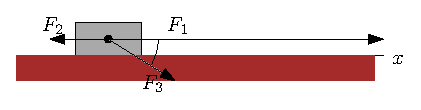
\includegraphics{img/disco.eps}
    \caption{Disco da hockey e vettori}
    \label{fig:hockeyevett}
  \end{figure}
  un disco da hockey si muove su una superficie ghiacciata priva di attrito lungo l'asse x in un moto unidirezzionale. La sua massa è $m=0.20kg$. Le forze $F_1$ ed $F_2$ di modulo rispettivamente 4.0N e 2.0N, agiscono lungo l'asse. Una terza forza $F_3$ di modulo 1.0N forma un angolo di $30^o$ rispetto all'asse x. In ciascuno dei tre casi qual è l'accelerazione del disco?
\end{es}
\begin{sol}
  In questo caso usuamo la seconda legge di Newton usando la formula della forza netta agente su un corpo, qui di forza c'è ne più di una quindi bisogna valutare le singole forze per poi calcolare l'accelerazione totale.
  \begin{eqnarray*}
    \vec{F}_{net}=m\vec{a} & \to{} & F_{net_x}=ma_x 
  \end{eqnarray*}
  Quindi se vogliamo trovare la forza di x dobbiamo fare una sommatoria:
  \begin{equation*}
    \sum F_x=ma_x
  \end{equation*}
  Da questo punto in poi dobbiamo calcolare $a_1x$ e $a_{2_1}$, visto che comunque il metodo migliore è procedere per punti con questo tipo di calcoli possiamo procedere nel seguente modo, creare un elenco ordinato e procedere in questo modo per evitare inutili disordini.
  \begin{enumerate}
  \item In primo luogo, conviene fare un veloce riepilogo delle variabili, quindi abbiamo 3 vettori/forze in gioco su questo corpo:
    \begin{equation*}
      \begin{cases}
        F_1=4.0N\\
        F_2=2.0N\\
        F_3=1.0N
      \end{cases}
    \end{equation*}
    con questo possiamo iniziare a lavorare sulle su $F_{1x}=ma_1x$ e $a_1x$.
    \begin{equation*}
      a_1x=\frac{F_{1x}}{m}=\frac{4N}{0.2kg}=20\frac{m}{s^2}
    \end{equation*}
  \item Visto che comunque $F_2$ ha vettorialmente un verso opposto a $F_1$ e quindi presenterà pure un segno algebrico opposto. Detto questo possiamo impostare la sommatoria $\sum F= F_{1x}-F_{2x}=ma_{2,1x}$
    \begin{equation*}
      a_{2_1}= \frac{F_{1x}-F_{2x}}{m}= \frac{4-2}{0.2}=\frac{2}{0.2}=10\frac{m}{s^2}
    \end{equation*}
  \item In extremis facciamo la somma vettoriale tra $F_2$ e $F_3$, quindi con la stessa formula usata prima possiamo calcolare anche questo caso\dots{}
    \begin{equation*}
      \sum F= -F_2x+F_2x=-2+1\cos30^o
    \end{equation*}
    $F_3$ ha un angolo di $30^o$ ed è contrassegnato con il simbolo $\uptheta$ e con questo abbiamo soddisfatto i requisiti posti dal testo.
  \end{enumerate}
\end{sol}
\clearpage
\begin{es}
  Un auto che slitta su una strada ghiacciata. Confrontiamo qui i tipici spazi di arresto necessari per fermarsi da una velocità iniziale di 10.0m/s su asfalto asciutto, fondo orizzontale ghiacciato e una strada gelata in discesa.
  \begin{figure}[ht!]
    \centering
    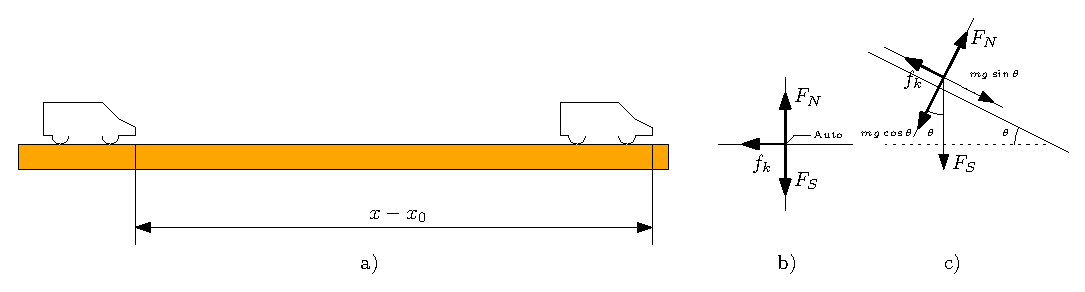
\includegraphics[scale=0.9]{img/auto.eps}
    \caption{Automobile su strada}
    \label{fig:autosust}
  \end{figure}
  \begin{tasks}
    \task Qual'è lo spazio d'arresto per un'auto su un piano orizzontale (come in figura \ref{fig:autosust}a) se il coefficiente di attrito è $\mu_k=0.60$, un valore tipico per pneumatici ordinari su asfalto asciutto? Trascuriamo gli effetti dell'aria, supponiamo che le ruote siano bloccate e che striscino sull'asfalto. Tracciamo l'asse $x$ nella direzione del moto.
    \task Quanto diventa lo spazio di frenata in condizioni di strada ghiacciata con $\mu_k=0,10$?
  \end{tasks}
\end{es}
\begin{sol}
  Questo tipo di esercizio è già partizionato in punti quindi è il caso di procedere nello stesso modo, con un altro elenco ordinato.
  \begin{tasks}
    \task Per svolgere il primo punto sarà necessaria la formula della forza netta agente su un corpo
    \begin{equation*}
      \begin{matrix}
        -f_k=ma_x &\to& -\mu_kF_N=ma_x\\
        -\mu_k\not{m}g=\not{m}a_x&\to& a_x=-\mu_kg
      \end{matrix}
    \end{equation*}
    adesso andiamo a ricavare $x-x_0$, sapendo che $v_f=0$ e $v_0=10\frac{m}{s}$
    \begin{equation*}
      x-x_0=\frac{v_f^2-v_0^2}{2a_x}=8.5m
    \end{equation*}
    Quindi dopo questo sappiamo che la risposta corretta alla domanda è che $x-x_0=8.5m$, con questo si può passare al secondo punto posto.
    \task per calcolare lo psazio di frenata su una strada ghiacciata basterà semplicemente utilizzare la stessa formula vista prima per il calcolo di $x-x_0$, con la differenza che al denominatore al posto di $a_x$ ci sarà $2\mu_kg$ e anche il fatto che unico vettore interessato è $v_0$.
    \begin{equation*}
      x-x_0=\frac{v_0^2}{2\mu_kg}=\frac{\left(10\frac{m}{s}\right)}{20.1\cdot 9.81}=51m
    \end{equation*}
    Dopo questo possiamo dire che lo spazio di frenata che avrà l'automobile su una strada ghiacciata è di 51m sicuramente molto superiore a quella precedentemente osservata (la frenata è circa 6 volte più lenta rispetto a quella che si ottiene in una strada asciutta).
  \end{tasks}
\end{sol}
\begin{es}
  Un cannone posizionato su un monte alto 1 km spara un proiettile con un angolo di $35^o$ rispetto all’orizzontale. Il proiettile cade sulla vicina valle ad una distanza orizzontale $d= 3 km$. A quale velocità iniziale è stato sparato il proiettile? Qual è il tempo di volo?
\end{es}
\begin{sol}
  Vista la situazione il primo punto da svolgere è proprio quello di andare a definire delle variabili:
  \begin{eqnarray*}
    \theta= 35^0\\
    h=1km\\
    d=3km
  \end{eqnarray*}
  adesso dobbiamo andare a definire la distanza, andando a stilare un sistema con due funzione:
  \begin{eqnarray*}
    \begin{cases}
      x-x_0=d=(v_0\cos\theta_0)t\\
      y-y_0=-h=(v_0\sin\theta_0)t-\frac{1}{2}gt^2
    \end{cases}
  \end{eqnarray*}
  ora, dopo aver ricavato la distanza possiamo andare a definire il tempo:
  \begin{eqnarray*}
    \begin{cases}
      t=\frac{d}{v_0\cos\theta_0}\\
      -h=(v_0\sin\theta_0)\frac{d}{v_0\cos\theta_0}-\frac{g}{2}\cdot \frac{d^2}{v_0^2\cos\theta_0}
    \end{cases}
  \end{eqnarray*}
  ora a questo punto possiamo andare a definire $v_0$:
  \begin{eqnarray*}
    v_0^2\sin\theta_0\cos\theta_0d=\frac{gd^2}{2}+hv_0^2\cos^2\theta_0=0\\
    v_0^2=\frac{gd^2}{2(\sin\theta\cos\theta_0d+h\cos\theta_0)}\\
    v_0=\sqrt{\frac{gd^2}{2(\sin\theta\cos\theta_0d+h\cos\theta_0)}}
  \end{eqnarray*}
\end{sol}
\subsection{Moto circolare univorme}
\label{sec:motciruni}
\begin{es}
  I tratti curvilinei delle autostrade sono spesso inclinati per limitare l'effetto di sbandamento verso l'esterno. Con pavimentazione asciutta la forza d'attrito tra strada e pneumatico è di norma largamente sufficiente
  \begin{figure}[ht!]
    \centering
    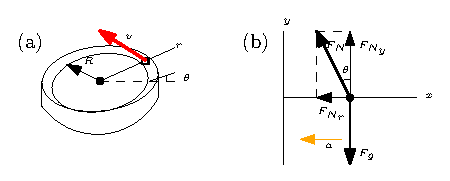
\includegraphics{img/perc.eps}
    \caption{Curvilineo del autostrada}
    \label{fig:curvl}
  \end{figure}
  a prevenire slittamenti. Ad asfalto bagnato, invece, l'attrito si riduce e l'inclinazione del pianostradale diventa importante. Nella figura \ref{fig:curvl}a è disegnata un'automobile di massa $m$ che percorre alla velocità di 20m/s un tratto curvo inclinato di raggio R=190m. Si tratta di una macchina ordinaria, non di formula 1, e quindi la portanza negativa esaminata nel proglema svolto precedentemente è trascurabile. Ignorando la forza d'attrito, quale angolo d'inclinazione $\theta$ del piano stradale eviterebbe la fuoriuscita dalla carreggiata?
\end{es}
\begin{sol}
  In questo caso bisogna comunque analizzare le forze in gioco in questo caso infatti come si vede nel \ref{fig:curvl}b, le forze in atto sono sostanzialmente $F_N$ che agisce vettorialmente sulla superficie della strade inclinata di un angolo $\theta$ quindi viene suddiviso nei vettori $F_{N_y}$ e $F_{N_r}$ che corrispondono a:
  \begin{equation*}
    \begin{matrix}
      F_{N_x}=F_N\cos\theta\\
      F_{N_y}=F_N\sin\theta
    \end{matrix}
  \end{equation*}
  La forza di Graviota $F_g$. Detto questo possiamo usare le consuete formule precedentemente utilizzate aggiungento quelle inerenti al moto circolare uniforme.
  \begin{equation*}
    \begin{matrix}
      y & F_N\cos\theta-mg=0 & \to & \vec{F}_N\cos\theta=m\vec{g}\\
      x & -F_N\sin\theta=m\left(-\frac{v^2}{R}\right) && \frac{\not{F}_N\sin\theta}{\not{F}_N\cos\theta}=\frac{\not{m}v^2}{\not{m}Rg}\\
      & F_N\sin\theta=\frac{v^2}{R}
    \end{matrix}
  \end{equation*}
  fatto questo possiamo ricavarci l'angolo di curvatura $\theta$ con la seguente formula:
  \begin{equation*}
    \frac{\sin\theta}{\cos\theta}=\frac{v^2}{Rg}\to \tan\theta=\frac{v^2}{Rg} \to \theta=\arctan\left(\frac{v^2}{Rg}\right)
  \end{equation*}
  In questo caso si tratta di andare a trasformare il $\frac{\sin\theta}{\cos\theta}$ in $tan\theta$ che poi con poi messo sotto frazione più esser trasformato in $\arctan$.
\end{sol}

\section{Oscillazioni}
\label{sec:oscill}

\subsection{Oscillatore armonico smorzato}
\label{sec:osciarmsmo}

\begin{es}
  Per l'oscillatore smorzato riportato nello schema, ipotizziamo una massa del blocco pari a $m=250g$, una costante elestica della molla $k=85 N/m$ e costante di smorzamento pari a $b=70\frac{g}{s}$.
  \begin{itemize}
  \item Qual è il periodo del moto?
  \item In quanto tempo l'ampiezza dell'oscillazione smorzata si riduce a metà del valore iniziale?
  \item Quanto tempo impiega l'energia meccanica per ridursi di metà del valore iniziale?
  \end{itemize}
\end{es}
\begin{sol}
  Ora l'esercizio è suddiviso in punti quindi l'approccio più spontaneo come visto negli esercizi precedenti:
  \begin{itemize}
  \item Verifichiamo il livello di smorzamento:
    \begin{equation*}
      \begin{matrix}
        b= 0.07\frac{kg}{s} << \sqrt{\frac{k}{m}}=4.6\frac{kg}{s}\\
        T=2\pi \sqrt{\frac{m}{k}}=0.34s
      \end{matrix}
    \end{equation*}
  \item Partendo dalla relazione
    \begin{equation*}
      x(t)=x_me^{-\frac{bt}{2m}}\cos\left(\omega_{sm}t+\phi\right)
    \end{equation*}
    l'ampiezza dell'oscillazione sarà $x_me^{-\frac{bt}{2m}}$. Imponiamo
    \begin{equation*}
      \begin{matrix}
        x_me^{-\frac{bt}{2m}}=\frac{x_m}{2=-\frac{bt}{2}}\Rightarrow{}-\frac{bt}{2m}=\ln\left(\frac{1}{2}\right)\Rightarrow{} t=\frac{2m\ln(0.5)}{b}=5s\\
        \frac{1}{2}kx_m^2e^{\frac{-bt}{m}}=\frac{1}{2}\left(\frac{1}{2}kx_m^2\right)\Rightarrow{}-\frac{bt}{m}=\ln(0.5)\Rightarrow{}2.5s
      \end{matrix}
    \end{equation*}
  \end{itemize}
  e con questo l'esercizio è stato svolto.
\end{sol}

\subsection{Moti elastici}
\label{sec:motielastici}

\begin{es}
  Un sistema oscillante blocco-molla ha energia meccanica di 1.00J, ampiezza 10.0cm e velocità massima $11.00\frac{m}{s}$. Trovate:
  \begin{tasks}
    \task la costante elastica;
    \task la massa del blocco;
    \task la frequenza di oscillazione.
  \end{tasks}
\end{es}
\begin{sol}
  L'energia meccanica è dato da $K+U=1J$. Nel punto di massima compressione c'è solo un'energia elastica
  \begin{equation*}
    \begin{matrix}
      \frac{1}{2}kx^2=1J\\
      k=\frac{2J}{x^2}=\frac{2J}{(0.1m)^2}=\boxed{200\frac{N}{m}}
    \end{matrix}
  \end{equation*}
  La massa del blocco si può trovare studiando il sistema nel punto in cui la sua velocità è massima: qua, infatti, non c'è energia potenziale elastica:
  \begin{equation*}
    \frac{1}{2}mv^2_{max}=1J \to m=\frac{2J}{v^2_{max}}=\frac{2J}{(11.2m/s)^2}=\boxed{0.016}Kg
    \end{equation*}
    La frequenza $f$ è data da:
    \begin{equation*}
      f=\frac{1}{2\pi}\sqrt{\frac{k}{m}}=\boxed{17.79Hz}
    \end{equation*}
    e con questo l'esercizio è concluso\dots
\end{sol}
\begin{es}
  Trovate l'energia meccanica di un sistema blocco-molla con costante elastica di 1.3 N/cm e ampiezza di oscillazione di 2.4cm.
\end{es}
\begin{sol}
  In questo caso dobbiamo solo calcolare l'energia E, in modo abbastanza semplice, tramite la formula $E=\frac{1}{2}kx^2$, nel seguente modo:
  \begin{equation*}
    E=\frac{1}{2}kx^2=\frac{1}{2}\cdot(130N/m)\cdot(0.024m)^2=0.037J
  \end{equation*}
  e questo l'esercizio è concluso.
\end{sol}
\begin{es}
  Un blocco di massa $M=5.4kg$, a riposo su un piano orizzontale privo di attrito, è ancorato a un punto fisso tramite una molla di costanza $k=6000N/m$. Un proiettile di massa m=9.5g e velocità $v$ di modulo $630m/s$ colpisce il blocco Mm restando incastrato nel blocco. Determinare
  \begin{tasks}
    \task la velocità del blocco immediatamente dopo l'urto;
    \task l'ampiezza del moto armonico semplice risulta, assumendo che la compressione della molla sia trascurabile finché il proiettile non sia cmpletamente incastrato.
  \end{tasks}
\end{es}
\begin{sol}
  L'urto è anelastico, $\vec{p}$ si conserva e troviamo $v_f$
  \begin{equation*}
    \begin{matrix}
      m_pv_p=(M+m_p)v_f\\
      v_f=\frac{m_pv_p}{M+m_p}=\frac{0.0095kg\cdot 630m/s}{5.4kg+0.0095kg}=\boxed{1.1m/s}
    \end{matrix}
  \end{equation*}
  L'energia si conserva:
  \begin{equation*}
    \begin{matrix}
      \frac{1}{2}(M+m_p)v_f^2=\frac{1}{2}kx^2\\
      x=\sqrt{\frac{(M+m_p)v_f^2}{k}}=\boxed{0.033m}
    \end{matrix}
  \end{equation*}
  e con questo l'esercizio è terminato.
\end{sol}
\begin{es}
  Due blocchi (m = 1.0kg e M = 10kg) e una molla (k = 200N/m) sono sistemati una sopra l'altra, con m sopra M su una superficie orizzontale priva di attrito. Il coefficiente di attrito statico fra i due blocchi è di 0.40. Quel'è la massima ampiezza del moto armonico semplice ammissibile per evitare lo slitamento tra i due blocchi?
\end{es}
\begin{sol}
  Il blocco sta fermo fintanto che la forza ``laterale'' subito non supera lo forza d'attrito statico. L'accelerazione massima durante il moto armanico è data da:
  \begin{equation*}
    a_{max}=\omega^2x
  \end{equation*}
  con $\omega = \sqrt{\frac{k}{M_{tot}}}=\sqrt{\frac{200N/m}{11kg}}=4.26Hz$, Vogliamo che $m\cdot a_{max}$ non superi la forza d'attrito:
  \begin{equation*}
    \begin{matrix}
      m\cdot a_{max}=mg\cdot \mu\\
      m\cdot \omega^2x=mg\cdot \mu\\
      x = \frac{\mu g}{\omega^2}=\frac{0.4\cdot 9.81m/s^2}{(4.26Hz)^2}=\boxed{0.21m}
    \end{matrix}
  \end{equation*}
  E con questo l'esercizio è terminato con tutti i punti soddisfatti.
\end{sol}
\begin{es}
  Un pendolo di lunghezza 1.2m che oscilla muovendosi di moto armonico, è portato su un altro pianeta. Quando viene messo in funzione si osserva che il pendolo compie 100 oscilazioni complete in 280s. Quel'è dunque l'accelerazione di graviotà su quel pianeta?
\end{es}
\begin{sol}
  In primo luogo è giusto evidenziare quelli che sono i nostri dati:
  \begin{equation*}
    \begin{matrix}
      L=1.2m & \Delta t=280s\\
      T=2\pi \sqrt{\frac{L}{a}}& N_0=100
    \end{matrix}
  \end{equation*}
  dopo aver fatto questo possiamo andare a ricavarci T, con il seguente sviluppo
  \begin{equation*}
    T=\frac{\Delta t}{N_0}=\frac{280s}{100}=2.8s
  \end{equation*}
  Una volta aver fatto questo possiamo ricavare $a$ nel sequente modo:
  \begin{equation*}
    \frac{T^2}{4\pi^2}\Rightarrow{} a=\frac{4\pi^2L}{T^2}=\frac{4\pi^2\cdot1.2m}{(2.8s)^2}=6.04\frac{m}{s^2}
  \end{equation*}
\end{sol}
\begin{es}
  Un pendolo semplice lungo 2m è posto all'interno di un ascensore. Calcolare la frequenza di oscillazione nei seguenti casi:
  \begin{enumerate}
  \item l'ascensore è fermo;
  \item l'ascensore sta salendo con un'accelerazione pari a $2m/s^2$
  \item l'ascensore è in caduta libera
  \end{enumerate}
\end{es}
\begin{sol}
  In primo luogo andiamo a riportare i dati, come ad esempio la lunghezza:
  \begin{equation*}
    L=2m
  \end{equation*}
  adesso dopo aver segnato i dati, possiamo procedere a svolgere i tre casi presentati:
  \begin{enumerate}
  \item Se l'ascensore è fermo avremmo un $T=2\pi \sqrt{\frac{g}{L}}$ e per calcolare frequenza $f=\frac{1}{T}$, per avere l'idea chiara in Hz dobbiamo procedere nel seguente modo:
    \begin{equation*}
      f=\frac{1}{2\pi}\sqrt{\frac{g}{2}}=\frac{1}{2\pi}\sqrt{\frac{9.81\frac{\not{m}}{s^2}}{2\not{m}}}=0.35\frac{1}{s}=0.35Hz
    \end{equation*}
    
  \item Adesso valutiamo il caso in cui l'ascensore sia in movimento, salendo ad una velocità di $2m/s^2$, in questo caso, infatti, una forza a che avrà un effetto verticale sul pendolo, oltre alla forza peso, infatti $a_{tot}$ sarà composto dalla forza peso e da questa ulteriore forza $a$.
    \begin{equation*}
      a_{tot}=g+{\color{red}a}
    \end{equation*}
    quindi andando ad adattare la formula vista nel primo caso alla nuova situazione avremmo:
    \begin{equation*}
      f=\frac{1}{2\pi}\sqrt{\frac{g+a}{L}}=\frac{1}{2\pi}\sqrt{\frac{9.81\frac{\not{m}}{s^2}+2\frac{\not{m}}{s^2}}{2\not{m}}}=0.39Hz
    \end{equation*}
  \item Per ultimo punto troviamo l'ascensore in caduta libera, in questo caso avremmo un $a_{tot}= 0$ e per forza di cose $T\to +\infty$, nel esempio in questione è presente solo una forza $\vec{g}$ e quindi:
    \begin{equation*}
      f=0
    \end{equation*}
    In questa perticolare condizione non avviene un moto oscillatorio.
  \end{enumerate}
\end{sol}
\begin{es}
  Un oscillatore armonico smorzato con una massa di 235g è soggetto a una forza di attrito caratterizzata da una costante $\gamma=2.2s^{-1}$.
  \begin{itemize}
  \item qual'è la forza di attrito che agisce sull'oscillatore quando la sua velocità è 2.8cm/s?
  \end{itemize}
\end{es}
\begin{sol}
  In primo luogo riportiamo sotto forma di fariabili i valori necessari a svolgere gli esercizi e convertiamole in un formato adeguato allo svolgimento delle formule:
  \begin{eqnarray*}
    m=235g=0.235kg & \gamma=2.2s^{-1}\\
    v=2.8\frac{cm}{s}=2.8\times 10^{-2}\frac{m}{s}
  \end{eqnarray*}
  quindi andando a definire la forza totale possiamo anche dire che:
  \begin{equation*}
    -k\vec{x}-\beta \vec{v}=m\vec{a}=\vec{F}_{tot}
  \end{equation*}
  ora, possiamo andare a calcolare $\vec{F}_a$
  \begin{eqnarray*}
    \vec{F}_a=-\beta\vec{v}=-\gamma\cdot m\cdot \vec{v}\\
    \abs{\vec{F}_a}=\gamma\cdot m\cdot v= 2.2 s^{-1}\cdot 0.235kg\cdot2.8\times 10^{-2}\frac{m}{s}=1.4\cdot 10^{-2}N
  \end{eqnarray*}
\end{sol}
\begin{es}
  Un corpo di massa 230g si muove sotto l'azione di una molla con costante elastica $0.45N/m$. La forza di attrito che agisce sul corpo ha modulo direttamente proporzionale a quello della velocità con costante di proporzionalità $\beta=0.017N\cdot s/m$. Il corpo è inizialmente fermo lontano della posizione di equilibrio.
  \begin{itemize}
  \item Verifica che si ha uno smorzamento sottocritico.
  \end{itemize}
\end{es}
\begin{sol}
  Come sempre il primo passo è quello di andare ad esplicitare i dati necessari allo svolgimento del problema:
  \begin{eqnarray*}
    m=230g=0.23kg & k=0.45\frac{N}{m}\\
    \beta=0.017\frac{N\cdot s}{m}
  \end{eqnarray*}
  Per comprendere meglio l'esercizio è giusto fare una precesazione, i moti elastici smorzati si dividono in:
  \begin{center}
    \Tree[.Smorzamento [.sottoscritico $\gamma<2W$ ] [.sovrascritico $\gamma>2W$ ] ]
  \end{center}
  Quindi prendendo questo preconcetto possiamo proseguire, a noi servono i valori di $W$ e di $\gamma$, le formule per il calcolo sono:
  \begin{equation*}
    \begin{matrix}
      W=\sqrt{\frac{k}{m}} & \gamma =\frac{\beta}{m}
    \end{matrix} 
  \end{equation*}
  Detto questo andiamo a calcolare i due valori sostituendo le variabili in valori nomerici:
  \begin{equation*}
    \begin{matrix}
      W=\sqrt{\frac{0.45\frac{N}{m}}{0.23kg}}=1.40s^{-1}\\
      \gamma=\frac{0.017\frac{N\cdot s}{m}}{0.23kg}=0.07s^{-1}
    \end{matrix}
  \end{equation*}
  considerando i risultati possiamo dedurre che lo smorzamento è di tipo sottoscritico, visto che $\gamma<2W$.
\end{sol}
\end{document}
